\documentclass{article}
\usepackage[T1]{fontenc}
\usepackage[ansinew ]{inputenc}
\usepackage{amsmath}
\usepackage{tikz}
\usepackage{tikzsymbols}
\usepackage{lmodern}
\usepackage{xcolor}
\usetikzlibrary{arrows,automata}
\setlength\parindent{0pt}

\begin{document}

\begin{center}
  \Large{Informatik D - �bungsblatt 3}

  \large{Sebastian H�ffner, Andrea Suckro}
\end{center}



\section{Aufgabe 3.1}
Sei $L \subseteq \Sigma^{*}$ eine endliche Sprache, d.h. eine Sprache mit endlicher Anzahl W�rtern $\omega \in L$ endlicher L�nge. Dann k�nnen wir eine Grammatik definieren, die individuell alle W�rter aus $L$ generiert.
\begin{align*}
S\ \rightarrow\ \omega_i\ |\ \omega_{i+1}\ |\ ...
\end{align*}
Diese Grammatik kann in eine regul�re Grammatik �berf�hrt werden, indem jedes Wort $\omega_i$ als Verkettung von Regeln dargestellt wird.
\begin{align*}
S\ &\rightarrow\ O_{i,0}\ |\ O_{i+1,0}\ |\ ...\\
O_{i,0}\ &\rightarrow\ \omega_{i,0} O_{i,1} \\
O_{i,1}\ &\rightarrow\ \omega_{i,1} O_{i,2} \\
...
\end{align*}
In der Vorlesung wurde bereits gezeigt, dass regul�re Grammatiken in regul�re Ausdr�cke und endliche Automaten �berf�hrt werden k�nnen, also ist die endliche Sprache ebenfalls regul�r.



\section{Aufgabe 3.2}
\subsection{Aufgabe 3.2 (a)}
\begin{align*}
Z_1 &\rightarrow\ 1\ |\ 1Z_2 \\
Z_2 &\rightarrow\ 1\ |\ 1Z_2\ |\ 0Z_3 \\
Z_3 &\rightarrow\ 1\ |\ 0Z_1
%Z_4 &\rightarrow\ 
\end{align*}

\subsection{Aufgabe 3.2 (b)}
\begin{center}
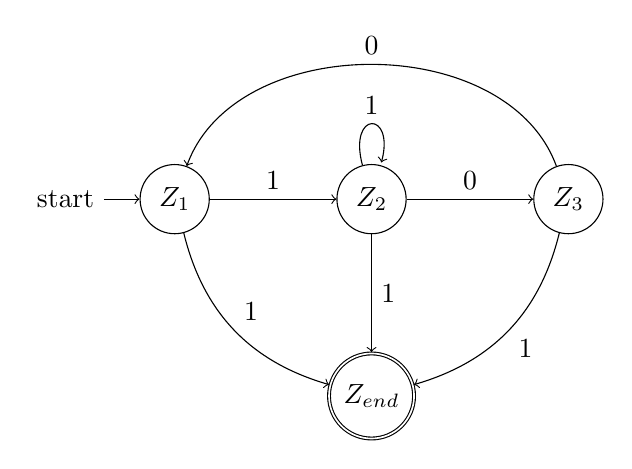
\begin{tikzpicture}[->, auto, node distance=2.5cm]
  \node[initial,state]   (Z1)               {$Z_1$};
  \node[state]           (Z2) [right of=Z1] {$Z_2$};
  \node[state]           (Z3) [right of=Z2] {$Z_3$};
  \node[state,accepting] (Ze) [below of=Z2] {$Z_{end}$};

  \path (Z1) edge [bend right]           node {1} (Ze)
             edge                        node {1} (Z2)
        (Z2) edge                        node {1} (Ze)
             edge [loop above]           node {1} (Z2)
             edge                        node {0} (Z3)
        (Z3) edge [bend left]            node {1} (Ze)
             edge [above, bend right=70] node {0} (Z1)
        ;
\end{tikzpicture}
\end{center}



\section{Aufgabe 3.3}
\begin{center}
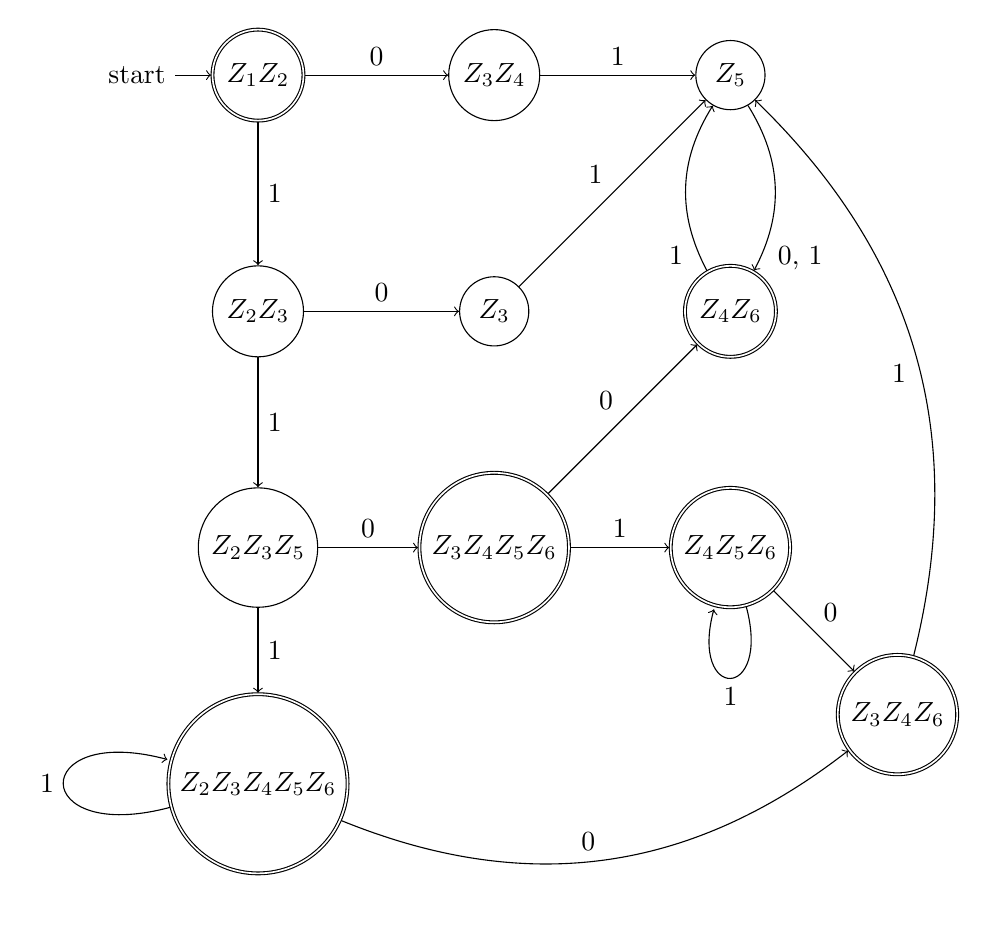
\begin{tikzpicture}[->, auto, node distance=3cm]
  \node[initial,state,accepting] (Z1Z2)                               {$Z_1Z_2$};
  \node[state]                   (Z2Z3)       [below of=Z1Z2]         {$Z_2Z_3$};
  \node[state]                   (Z2Z3Z5)     [below of=Z2Z3]         {$Z_2Z_3Z_5$};
  \node[state,accepting]         (Z2Z3Z4Z5Z6) [below of=Z2Z3Z5]       {$Z_2Z_3Z_4Z_5Z_6$};
  \node[state]                   (Z3)         [right of=Z2Z3]         {$Z_3$};
  \node[state]                   (Z3Z4)       [right of=Z1Z2]         {$Z_3Z_4$};
  \node[state,accepting]         (Z3Z4Z5Z6)   [right of=Z2Z3Z5]       {$Z_3Z_4Z_5Z_6$};
  \node[state,accepting]         (Z4Z5Z6)     [right of=Z3Z4Z5Z6]     {$Z_4Z_5Z_6$};
  \node[state,accepting]         (Z4Z6)       [right of=Z3]           {$Z_4Z_6$};
  \node[state]                   (Z5)         [right of=Z3Z4]         {$Z_5$};
  \node[state,accepting]         (Z3Z4Z6)     [below right of=Z4Z5Z6] {$Z_3Z_4Z_6$};

  \path (Z1Z2)       edge [] node {0} (Z3Z4)
                     edge [] node {1} (Z2Z3)
        (Z2Z3)       edge [] node {0} (Z3)
                     edge [] node {1} (Z2Z3Z5)
        (Z2Z3Z5)     edge [] node {0} (Z3Z4Z5Z6)
                     edge [] node {1} (Z2Z3Z4Z5Z6)
        (Z2Z3Z4Z5Z6) edge [bend right] node {0} (Z3Z4Z6)
                     edge [loop left]  node {1} (Z2Z3Z4Z5Z6)
        (Z3)         %edge [] node {0} ()
                     edge [] node {1} (Z5)
        (Z3Z4)       %edge [] node {0} ()
                     edge [] node {1} (Z5)
        (Z3Z4Z5Z6)   edge [] node {0} (Z4Z6)
                     edge [] node {1} (Z4Z5Z6)
        (Z4Z5Z6)     edge []           node {0} (Z3Z4Z6)
                     edge [loop below] node {1} (Z4Z5Z6)
        (Z4Z6)       %edge [] node {0} ()
                     edge [bend left, pos=0.2] node {1} (Z5)
        (Z5)         %edge [] node {0} (Z4Z6)
                     %edge [] node {1} (Z4Z6)
                     edge [bend left, pos=0.8] node {0, 1} (Z4Z6)
        (Z3Z4Z6)     %edge [] node {0} ()
                     edge [bend right] node {1} (Z5)
        ;
\end{tikzpicture}
\end{center}



\section{Aufgabe 3.4}
Wir betrachten zuerst die �u�erste Alternative: $($\colorbox{gray!25}{$(b|a)^*d$}$|$\colorbox{gray!25}{$c$}$)$. Unser NDEA bekommt also je einen $\epsilon$-�bergang zu $(b|a)^*d$ (beginnend bei $Z_2$) und $c$ (beginnend bei $Z_9$). Der Automat zu $c$ ist trivial:

\begin{center}
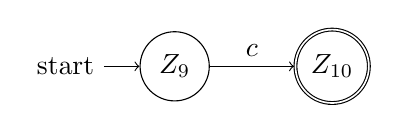
\begin{tikzpicture}[->, auto, node distance=2cm]
  \node[initial,state]   (Z9)                {$Z_9$};
  \node[state,accepting] (Z10) [right of=Z9] {$Z_{10}$};

  \path (Z9) edge node {$c$} (Z10)
        ;
\end{tikzpicture}
\end{center}

Der Teilautomat $(b|a)^*d$ ist etwas komplizierter. Zuerst hat er erneut eine Alternative: $($\colorbox{gray!25}{$b$}$|$\colorbox{gray!25}{$a$}$)$. 
Die Teilautomaten zu $b$ (beginnend bei $Z_3$) und $a$ (beginnend bei $Z_4$) sind wieder trivial:

\begin{center}
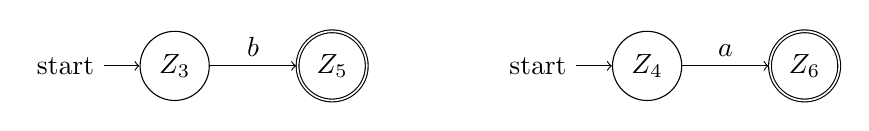
\begin{tikzpicture}[->, auto, node distance=2cm]
  \node[initial,state]   (Z3)               {$Z_3$};
  \node[state,accepting] (Z5) [right of=Z3] {$Z_5$};
  \node[initial,state]   (Z4) [right of=Z5, node distance=4cm] {$Z_4$};
  \node[state,accepting] (Z6) [right of=Z4] {$Z_6$};

  \path (Z3) edge node {$b$} (Z5)
        (Z4) edge node {$a$} (Z6)
        ;
\end{tikzpicture}
\end{center}

Um die Alternative $(b|a)$ darzustellen k�nnen wir diese beiden Teilautomaten mit $\epsilon$-�berg�ngen von Zustand $Z_2$ aus verkn�pfen (dabei �ndern sich die Start\-zu\-st�n\-de):

\begin{center}
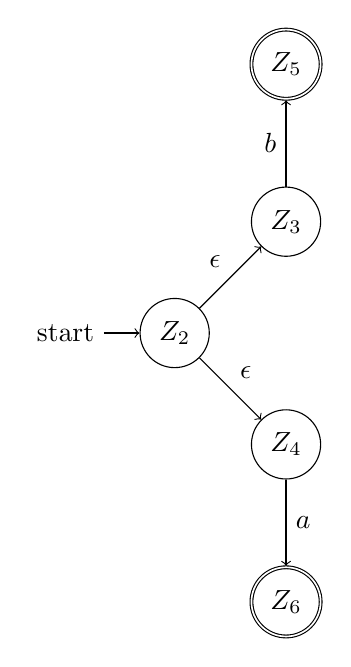
\begin{tikzpicture}[->, auto, node distance=2cm]
  \node[initial,state]   (Z2)                     {$Z_2$};
  \node[state]           (Z3) [above right of=Z2] {$Z_3$};
  \node[state,accepting] (Z5) [above of=Z3]       {$Z_5$};
  \node[state]           (Z4) [below right of=Z2] {$Z_4$};
  \node[state,accepting] (Z6) [below of=Z4]       {$Z_6$};

  \path (Z2) edge node {$\epsilon$} (Z3)
             edge node {$\epsilon$} (Z4)
        (Z3) edge node {$b$}        (Z5)
        (Z4) edge node {$a$}        (Z6)
        ;
\end{tikzpicture}
\end{center}

Als n�chstes k�nnen wir den Kleene-Stern dazu nehmen, um $(a|b)^*$ zu erhalten. Hierzu m�ssen wir den Automaten nur leicht erweitern und die Endzust�nde �ndern:

\begin{center}
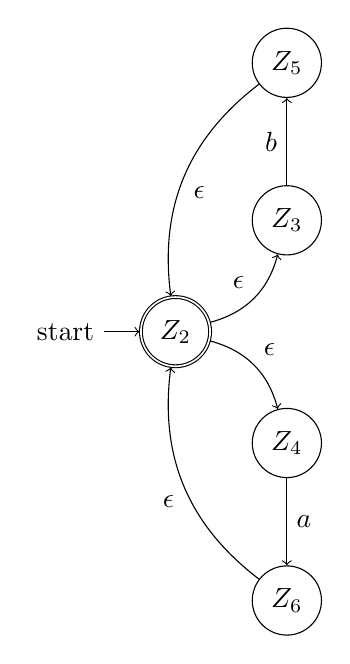
\begin{tikzpicture}[->, auto, node distance=2cm]
  \node[initial,state,accepting] (Z2)                     {$Z_2$};
  \node[state]                   (Z3) [above right of=Z2] {$Z_3$};
  \node[state]                   (Z5) [above of=Z3]       {$Z_5$};
  \node[state]                   (Z4) [below right of=Z2] {$Z_4$};
  \node[state]                   (Z6) [below of=Z4]       {$Z_6$};

  \path (Z2) edge [bend right] node {$\epsilon$} (Z3)
             edge [bend left]  node {$\epsilon$} (Z4)
        (Z3) edge              node {$b$}        (Z5)
        (Z4) edge              node {$a$}        (Z6)
        (Z5) edge [bend right] node {$\epsilon$} (Z2)
        (Z6) edge [bend left]  node {$\epsilon$} (Z2)
        ;
\end{tikzpicture}
\end{center}

Die Verkettung $(a|b)^*d$ folgt als n�chstes. Hierzu muss aus dem Endzustand des aktuellen Automaten ein $\epsilon$-�bergang zu einem weiteren trivialen Automaten, der $d$ akzeptiert, gezogen werden (und erneut der Endzustand verschoben werden).

\begin{center}
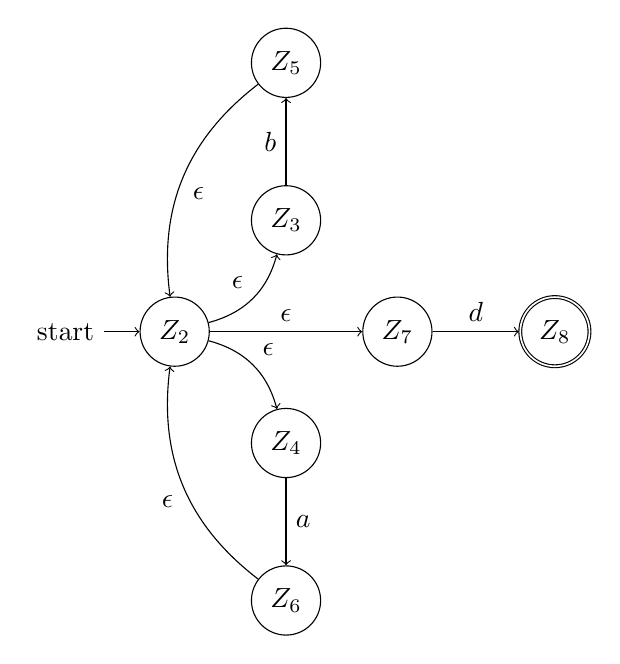
\begin{tikzpicture}[->, auto, node distance=2cm]
  \node[initial,state]   (Z2)                     {$Z_2$};
  \node[state]           (Z3) [above right of=Z2] {$Z_3$};
  \node[state]           (Z5) [above of=Z3]       {$Z_5$};
  \node[state]           (Z4) [below right of=Z2] {$Z_4$};
  \node[state]           (Z6) [below of=Z4]       {$Z_6$};
  \node[state]           (Z7) [below right of=Z3] {$Z_7$};
  \node[state,accepting] (Z8) [right of=Z7]       {$Z_8$};

  \path (Z2) edge [bend right] node {$\epsilon$} (Z3)
             edge [bend left]  node {$\epsilon$} (Z4)
        (Z3) edge              node {$b$}        (Z5)
        (Z4) edge              node {$a$}        (Z6)
        (Z5) edge [bend right] node {$\epsilon$} (Z2)
        (Z6) edge [bend left]  node {$\epsilon$} (Z2)
        (Z2) edge              node {$\epsilon$} (Z7)
        (Z7) edge              node {$d$}        (Z8)
        ;
\end{tikzpicture}
\end{center}

Als letzten Schritt k�nnen wir diesen Automaten und den Automaten vom Beginn ($c$, beginnend mit $Z_9$) erneut mit der Regel f�r Alternativen �ber Zustand $Z_1$ verkn�pfen:

\begin{center}
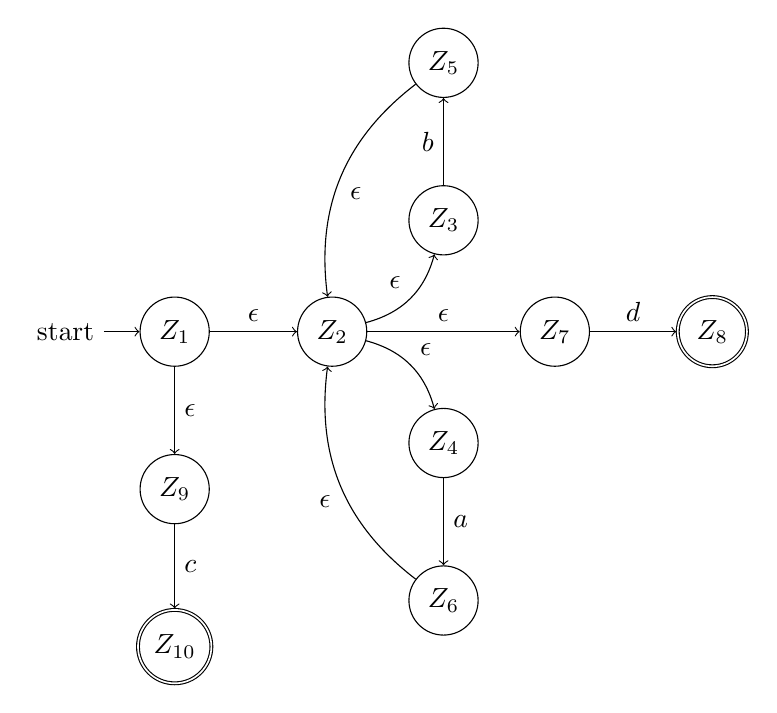
\begin{tikzpicture}[->, auto, node distance=2cm]
  \node[initial,state]   (Z1)                      {$Z_1$};
  \node[state]           (Z2)  [right of=Z1]       {$Z_2$};
  \node[state]           (Z3)  [above right of=Z2] {$Z_3$};
  \node[state]           (Z5)  [above of=Z3]       {$Z_5$};
  \node[state]           (Z4)  [below right of=Z2] {$Z_4$};
  \node[state]           (Z6)  [below of=Z4]       {$Z_6$};
  \node[state]           (Z7)  [below right of=Z3] {$Z_7$};
  \node[state,accepting] (Z8)  [right of=Z7]       {$Z_8$};
  \node[state]           (Z9)  [below of=Z1]       {$Z_9$};
  \node[state,accepting] (Z10) [below of=Z9]       {$Z_{10}$};

  \path (Z1) edge              node {$\epsilon$} (Z2)
        (Z1) edge              node {$\epsilon$} (Z9)
        (Z2) edge [bend right] node {$\epsilon$} (Z3)
             edge [bend left]  node {$\epsilon$} (Z4)
        (Z3) edge              node {$b$}        (Z5)
        (Z4) edge              node {$a$}        (Z6)
        (Z5) edge [bend right] node {$\epsilon$} (Z2)
        (Z6) edge [bend left]  node {$\epsilon$} (Z2)
        (Z2) edge              node {$\epsilon$} (Z7)
        (Z7) edge              node {$d$}        (Z8)
        (Z9) edge              node {$c$}        (Z10)
        ;
\end{tikzpicture}
\end{center}



\section{Aufgabe 3.5}
%\begin{figure}[h]
%  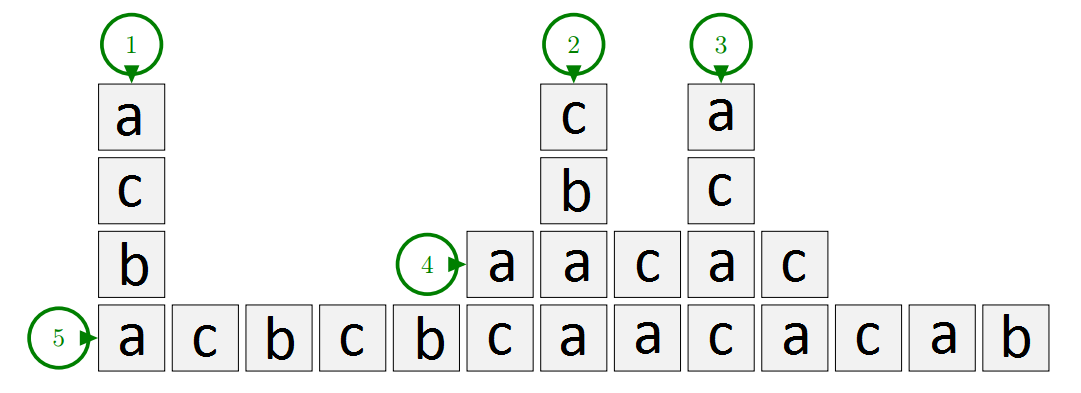
\includegraphics[width=\textwidth]{crossword.png}
%\end{figure}
\begin{enumerate}
	\item bbbbb
  \item bcbca
  \item bdda
  \item adadc
  \item bbaadd
\end{enumerate}



\section{Aufgabe 3.6}
% leeren auslassen? ist das der richtige approach? oder ist die Formel anders gemeint?
\begin{align*}
k=&0:\\
L_{i,j}^0&=\{\}\\
k=&1:\\
L_{1,1}^1&=\{\}\\
L_{1,2}^1&=\{b|\delta(Z_1,b)=Z_2\}\\
L_{1,3}^1&=\{a|\delta(Z_1,a)=Z_3\}\\
L_{1,4}^1&=\{\}\\
L_{2,1}^1&=\{\}\\
L_{2,2}^1&=\{\}\\
L_{2,3}^1&=\{\}\\
L_{2,4}^1&=\{\}\\
L_{3,1}^1&=\{\}\\
L_{3,2}^1&=\{\}\\
L_{3,3}^1&=\{a,b|\delta(Z_3,a)=Z_3,\delta(Z_3,b)=Z_3\}\\
L_{3,4}^1&=\{c|\delta(Z_3,c)=Z_4\}\\
L_{4,1}^1&=\{a|\delta(Z_4,a)=Z_1\}\\
L_{4,2}^1&=\{\}\\
L_{4,3}^1&=\{\}\\
L_{4,4}^1&=\{\}
\end{align*}
\begin{align*}
k=&2:\\
L_{1,1}^2&=\{\}\\
L_{1,2}^2&=\{\}\\
L_{1,3}^2&=\{a|\delta(Z_1,a)=Z_3\}\\
L_{1,4}^2&=\{ac|\delta(Z_1,a)=Z_3,\delta(Z_3,c)=Z_4\}\\
L_{2,1}^2&=\{\}\\
L_{2,2}^2&=\{\}\\
L_{2,3}^2&=\{\}\\
L_{2,4}^2&=\{\}\\
L_{3,1}^2&=\{ca|\delta(Z_3,c)=Z_4,\delta(Z_4,a)=Z_1\}\\
L_{3,2}^2&=\{\}\\
L_{3,3}^2&=\{aa,ab,ba,bb|\delta(Z_3,a)=Z_3,\delta(Z_3,b)=Z_3\}\\
L_{3,4}^2&=\{ac,bc|\delta(Z_3,a)=Z_3,\delta(Z_3,b)=Z_3,\delta(Z_3,c)=Z_4\}\\
L_{4,1}^2&=\{\}\\
L_{4,2}^2&=\{ab|\delta(Z_4,a)=Z_1,\delta(Z_1,b)=Z_2\}\\
L_{4,3}^2&=\{aa|\delta(Z_4,a)=Z_1,\delta(Z_1,a)=Z_3\}\\
L_{4,4}^2&=\{\}
\end{align*}
\begin{align*}
k=&3:\\
L_{1,1}^3&=\{aca|\delta(Z_1,a)=Z_3,\delta(Z_3,c)=Z_4,\delta(Z_4,a)=Z_1\}\\
L_{1,2}^3&=\{\}\\
L_{1,3}^3&=\{aaa,aab,aba,abb|\delta(Z_1,a)=Z_3,\delta(Z_3,a)=Z_3,\delta(Z_3,b)=Z_3\}\\
L_{1,4}^3&=\{aac,abc|\delta(Z_1,a)=Z_3,\delta(Z_3,a)=Z_3,\delta(Z_3,b)=Z_3,\delta(Z_3,c)=Z_4\}\\
L_{2,1}^3&=\{\}\\
L_{2,2}^3&=\{\}\\
L_{2,3}^3&=\{\}\\
L_{2,4}^3&=\{\}\\
L_{3,1}^3&=\{aca,bca|\delta(Z_3,a)=Z_3,\delta(Z_3,b)=Z_3,\delta(Z_3,c)=Z_4,\delta(Z_4,a)=Z_1\}\\
L_{3,2}^3&=\{cab|\delta(Z_1,b)=Z_2,\delta(Z_3,c)=Z_4,\delta(Z_4,a)=Z_1\}\\
L_{3,3}^3&=\{aaa,aab,aba,abb,baa,bab,bba,bbb|\delta(Z_3,a)=Z_3,\delta(Z_3,b)=Z_3\}\\
L_{3,4}^3&=\{aac,abc,bac,bbc|\delta(Z_3,a)=Z_3,\delta(Z_3,b)=Z_3,\delta(Z_3,c)=Z_4\}\\
L_{4,1}^3&=\{\}\\
L_{4,2}^3&=\{\}\\
L_{4,3}^3&=\{aaa,aab|\delta(Z_3,a)=Z_3,\delta(Z_3,b)=Z_3,\delta(Z_1,a)=Z_3,\delta(Z_4,a)=Z_1\}\\
L_{4,4}^3&=\{aac|\delta(Z_4,a)=Z_1,\delta(Z_1,a)=Z_3,\delta(Z_3,c)=Z_4\}
\end{align*}
\begin{align*}
k=&4:\\
L_{1,1}^4&=\{aaca,abca|\\&\delta(Z_1,a)=Z_3,\delta(Z_3,a)=Z_3,\delta(Z_3,b)=Z_3,\delta(Z_3,c)=Z_4,\delta(Z_4,a)=Z_1\}\\
L_{1,2}^4&=\{acab|\delta(Z_1,a)=Z_3,\delta(Z_3,c)=Z_4,\delta(Z_4,a)=Z_1,\delta(Z_1,b)=Z_2\}\\
L_{1,3}^4&=\{aaaa,aaab,aaba,aabb,abaa,abab,abba,abbb|\\&\delta(Z_1,a)=Z_3,\delta(Z_3,a)=Z_3,\delta(Z_3,b)=Z_3\}\\
L_{1,4}^4&=\{aaac,aabc,abac,abbc|\\&\delta(Z_1,a)=Z_3,\delta(Z_3,a)=Z_3,\delta(Z_3,b)=Z_3,\delta(Z_3,c)=Z_4\}\\
L_{2,1}^4&=\{\}\\
L_{2,2}^4&=\{\}\\
L_{2,3}^4&=\{\}\\
L_{2,4}^4&=\{\}\\
L_{3,1}^4&=\{aaca,abca,baca,bbca|\\&\delta(Z_3,a)=Z_3,\delta(Z_3,b)=Z_3,\delta(Z_3,c)=Z_4,\delta(Z_4,a)=Z_1\}\\
L_{3,2}^4&=\{acab,bcab|\\&\delta(Z_3,a)=Z_3,\delta(Z_3,b)=Z_3,\delta(Z_3,c)=Z_4,\delta(Z_4,a)=Z_1,\delta(Z_1,b)=Z_2\}\\
L_{3,3}^4&=\{aaaa,aaab,aaba,aabb,abaa,abab,abba,abbb,baaa,\\&baab,baba,babb,bbaa,bbab,bbba,bbbb\\&\delta(Z_3,a)=Z_3,\delta(Z_3,b)=Z_3\}\\
L_{3,4}^4&=\{aaac,aabc,abac,abbc,baac,babc,bbac,bbbc|\\&\delta(Z_3,a)=Z_3,\delta(Z_3,b)=Z_3,\delta(Z_3,c)=Z_4\}\\
L_{4,1}^4&=\{aaca|\delta(Z_4,a)=Z_1,\delta(Z_1,a)=Z_3,\delta(Z_3,c)=Z_4\}\\
L_{4,2}^4&=\{\}\\
L_{4,3}^4&=\{aaaa,aaab,aaba,aabb|\\&\delta(Z_4,a)=Z_1,\delta(Z_1,a)=Z_3,\delta(Z_3,a)=Z_3,\delta(Z_3,b)=Z_3\}\\
L_{4,4}^4&=\{aaac,aabc|\\&\delta(Z_4,a)=Z_1,\delta(Z_1,a)=Z_3,\delta(Z_3,a)=Z_3,\delta(Z_3,b)=Z_3,\delta(Z_3,c)=Z_4\}
\end{align*}

I have no clue how the algorithm works, but this is a regex:
\begin{align*}
(b | (a(a|b)^*c a)^* a(a|b)^*c)
\end{align*}



\end{document}